\documentclass[12pt,a4paper]{article}
\usepackage[utf8]{inputenc}
\usepackage{graphicx}
\usepackage{color}
\usepackage[newfloat]{minted}
\usepackage{caption}


\title{CmpE321}
\author{Mustafa Enes Çakır}
\date{August 2017}


\begin{document}

\newenvironment{code}{\captionsetup{type=listing}}{}
\SetupFloatingEnvironment{listing}{name=Code}

\begin{titlepage}

\newcommand{\HRule}{\rule{\linewidth}{0.5mm}}

\center % Center everything on the page

%----------------------------------------------------------------------------------------
%   HEADING SECTIONS
%----------------------------------------------------------------------------------------

\textsc{\LARGE BOĞAZİÇİ UNIVERSITY}\\[1.5cm] % Name of your university/college
\textbf{\Large CMPE 321}\\[0.5cm] % Major heading such as course name
\textsc{\large PROJECT 3}\\[2cm] % Minor heading such as course title
\textsc{\large Summer 2017}\\[3cm] % Minor heading such as course title

%----------------------------------------------------------------------------------------
%   TITLE SECTION
%----------------------------------------------------------------------------------------

\HRule \\[0.4cm]
{ \huge \bfseries Airline Reservation System}\\[0.4cm] % Title of your document
\HRule \\[4cm]

%----------------------------------------------------------------------------------------
%   AUTHOR SECTION
%----------------------------------------------------------------------------------------

\Large Mustafa Enes ÇAKIR \\ [2cm] % Your name

%----------------------------------------------------------------------------------------
%   DATE SECTION
%----------------------------------------------------------------------------------------

{\large August 4, 2017}\\[2cm] % Date, change the \today to a set date if you want to be precise
\vfill % Fill the rest of the page with whitespace
\end{titlepage}

\tableofcontents{}

\break

\section{Introduction}
    It's an in-house web-based airlines reservation application. Administrators can generate general instances and employees make reservations for customers. They can select seat on plane easily.

    I was planning to implemented it with Laravel Framework. But Laravel is handling almost everything, such as \emph{SQL inception}. So, I decided to developed my own little PHP framework. I heavily inspired from Laravel.

    Entry point of my application is \emph{index.php}. After that point, my \emph{Router} handles routing. I have 3 important directory. \emph{App} directory contains project specific files, such as \emph{Models, Controller, Routes, Views}. \emph{Core} directory contains my framework classes, such as \emph{QueryBuilder, Auth, Router, Request}. \emph{Public} directory contains stylesheets, scripts etc.

\section{Interface}
    \begin{figure}[h!]
    \centering
    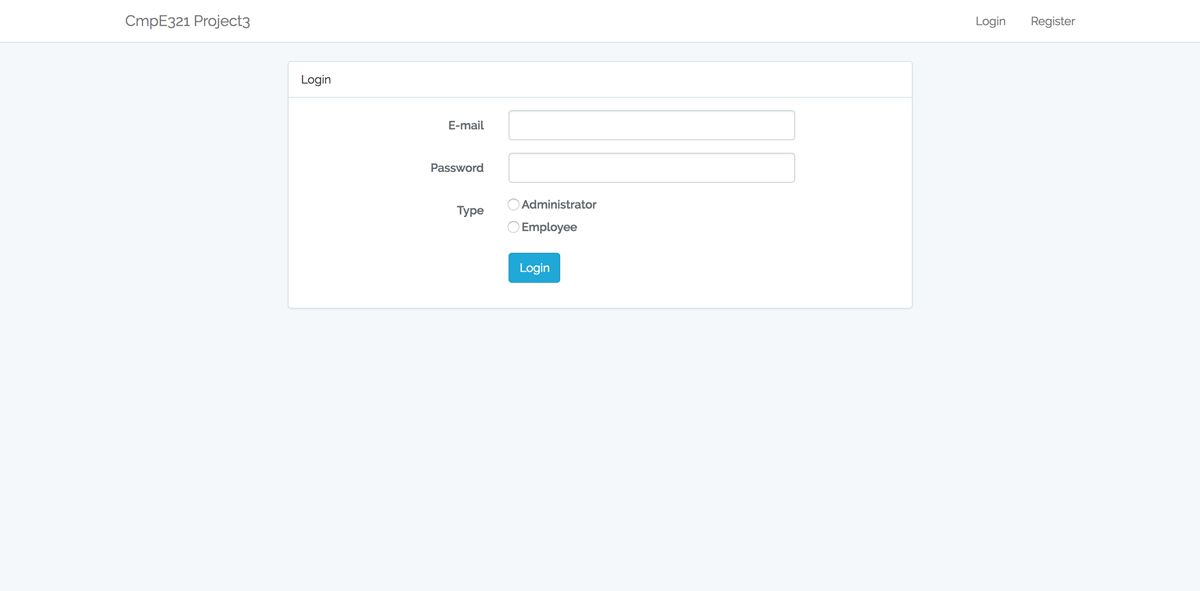
\includegraphics[width=135mm]{cmpe321_p3_ss1.png}
    \caption{Login Page for Administrators and Employees}
    \label{fig:ss1}
    \end{figure}

    \begin{figure}[h!]
    \centering
    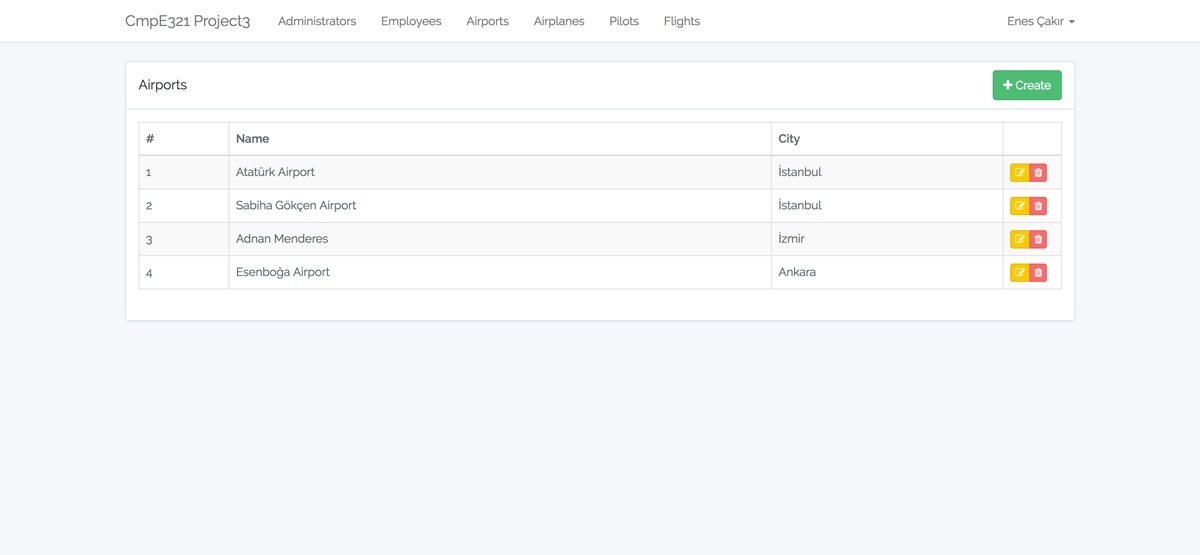
\includegraphics[width=135mm]{cmpe321_p3_ss2.png}
    \caption{Airport Listing Page}
    \label{fig:ss2}
    \end{figure}

    \begin{figure}[h!]
    \centering
    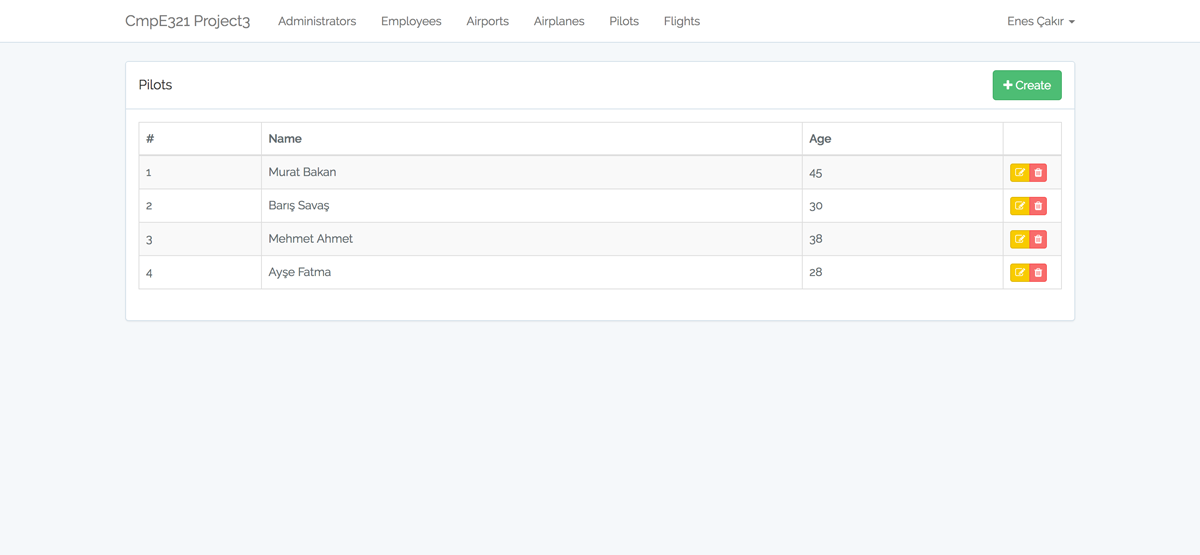
\includegraphics[width=135mm]{cmpe321_p3_ss3.png}
    \caption{Pilot Listing Page}
    \label{fig:ss3}
    \end{figure}

    \begin{figure}[h!]
    \centering
    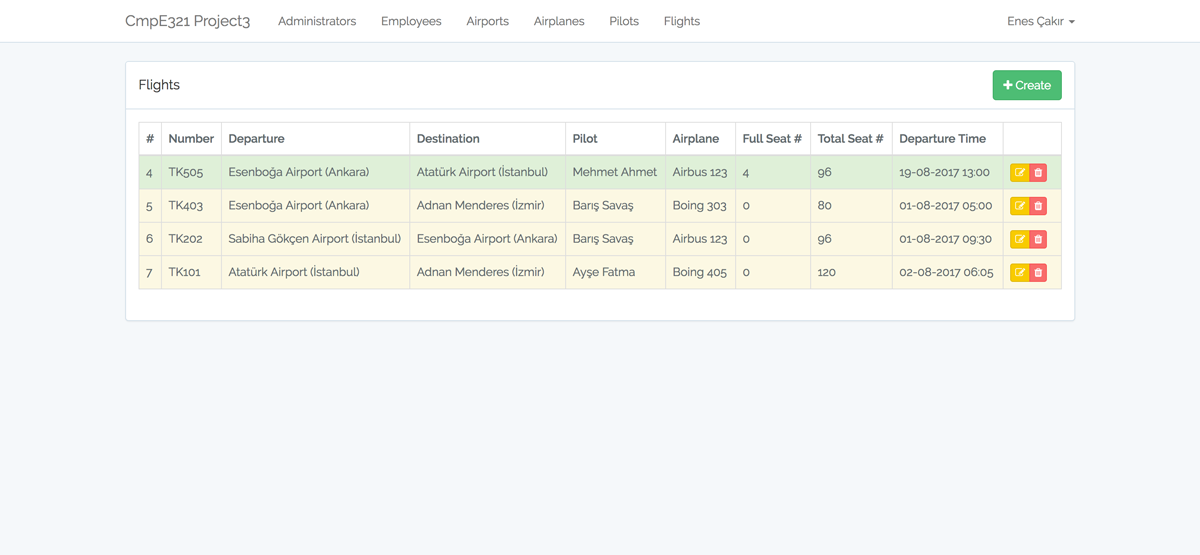
\includegraphics[width=135mm]{cmpe321_p3_ss4.png}
    \caption{Flight Listing Page}
    \label{fig:ss4}
    \end{figure}

    \begin{figure}[h!]
    \centering
    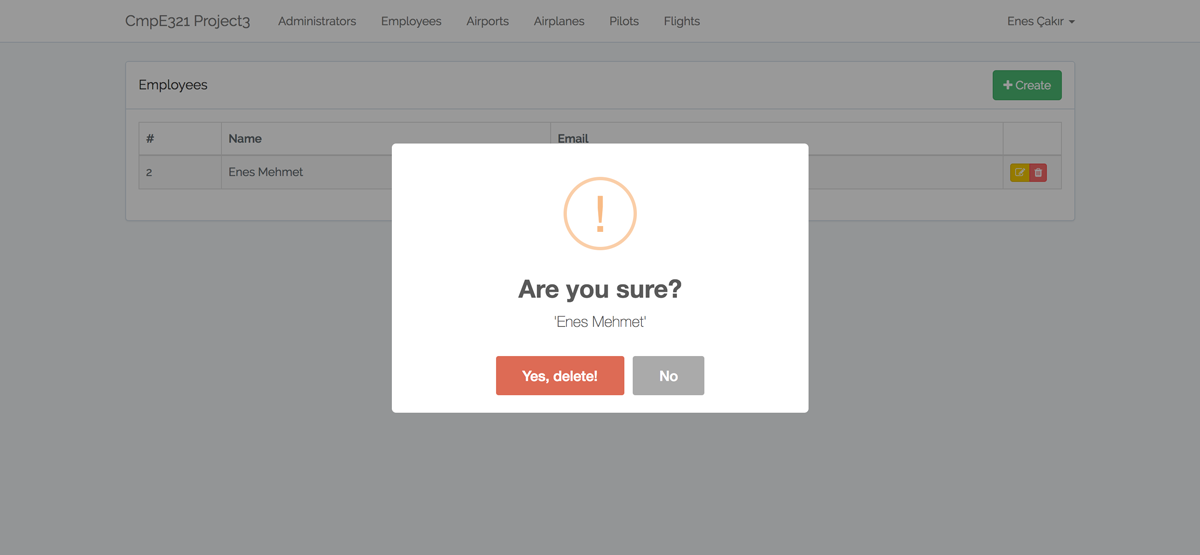
\includegraphics[width=135mm]{cmpe321_p3_ss5.png}
    \caption{Delete Confirmation Popup}
    \label{fig:ss5}
    \end{figure}

    \begin{figure}[h!]
    \centering
    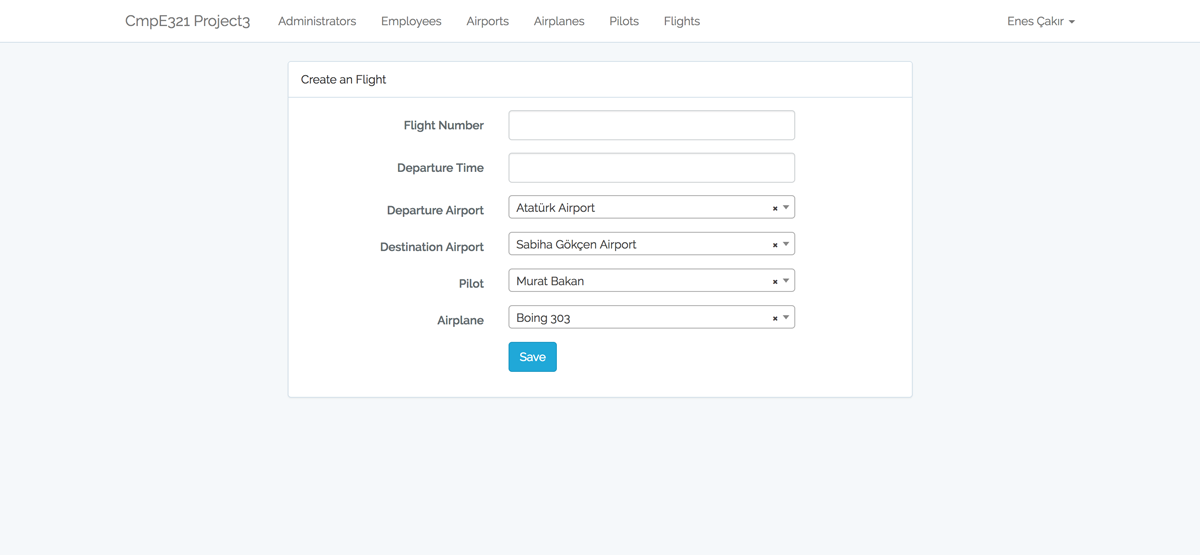
\includegraphics[width=135mm]{cmpe321_p3_ss6.png}
    \caption{Creating a Flight Page}
    \label{fig:ss6}
    \end{figure}

    \begin{figure}[h!]
    \centering
    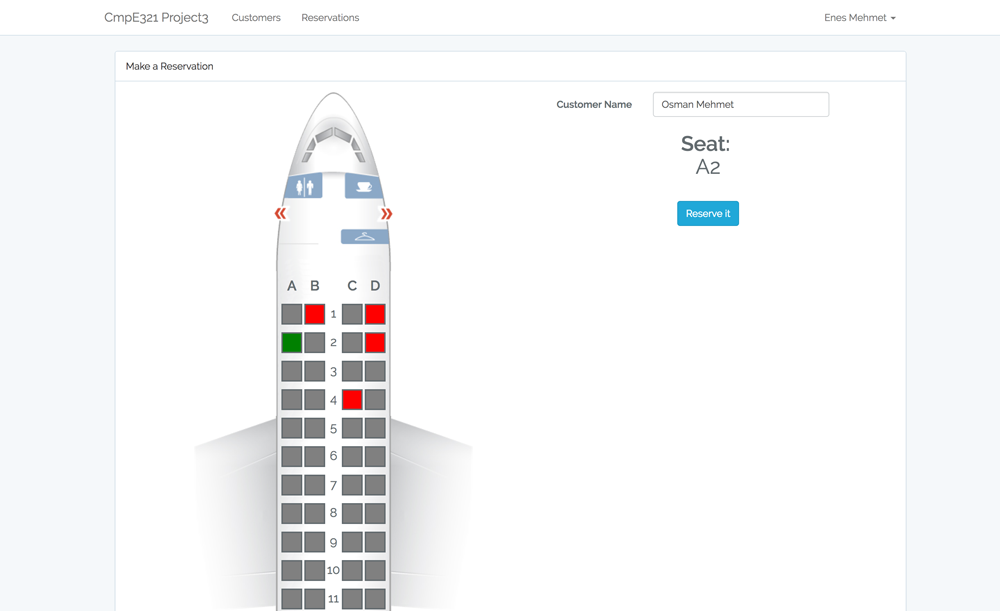
\includegraphics[width=135mm]{cmpe321_p3_ss7.png}
    \caption{Making Reservation Page}
    \label{fig:ss7}
    \end{figure}

    \clearpage

\section{Database}

\subsection{ER Diagram}
    \begin{figure}[h!]
    \centering
    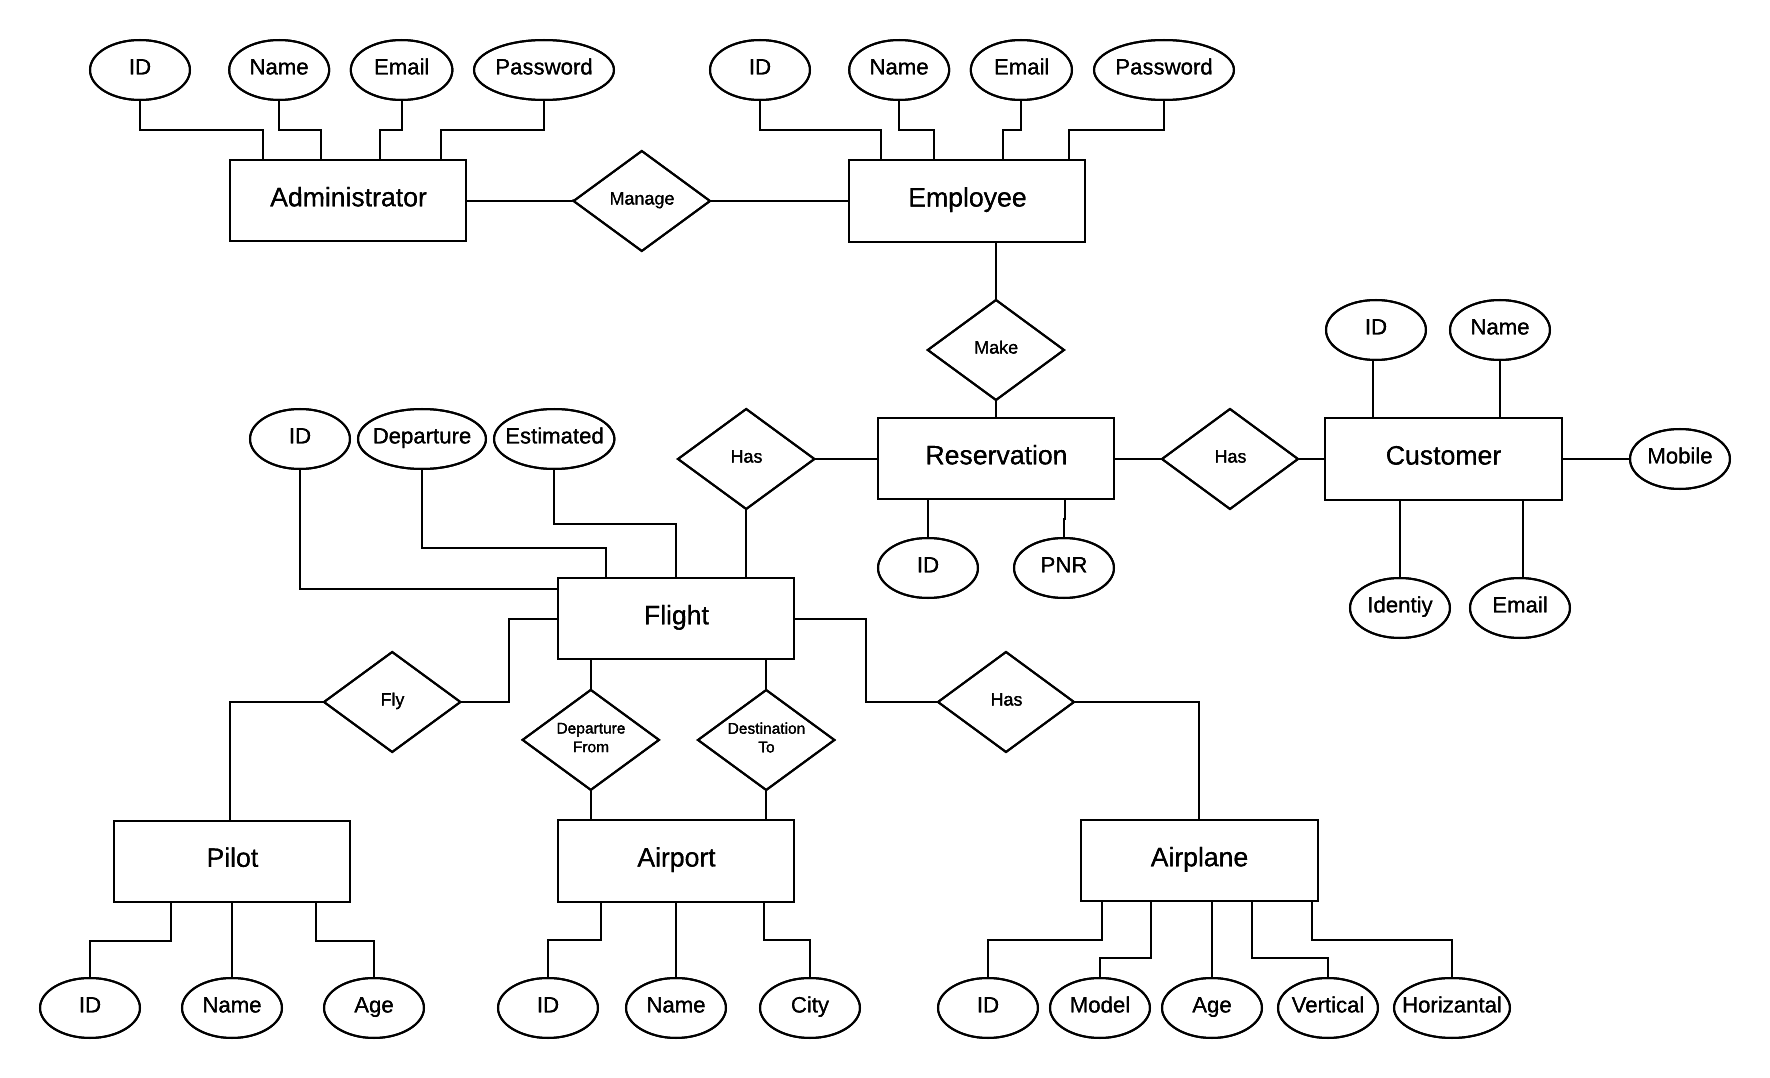
\includegraphics[width=135mm]{cmpe321_p3_ER.png}
    \caption{ER Diagram of Database}
    \label{fig:ss7}
    \end{figure}

\subsection{Procedures}
\begin{code}
\begin{minted}[mathescape, linenos, numbersep=5pt, gobble=2, frame=lines,framesep=2mm]{mysql}
    CREATE PROCEDURE `past_flights`(IN pid VARCHAR(10))
    BEGIN
        IF pid = "ALL" THEN
            SELECT f.*, des.name as des_name, des.city as des_city,
                dep.name as dep_name, dep.city as dep_city,
                p.name as p_name, ap.model as ap_model
            FROM flights as f
            JOIN airports as des ON des.id = f.destination_id
                JOIN airports as dep ON dep.id = f.departure_id
                JOIN pilots as p ON p.id = f.pilot_id
                JOIN airplanes as ap ON ap.id = f.airplane_id
                WHERE f.departured_at < NOW();
        ELSE
            SELECT f.*, des.name as des_name, des.city as des_city,
                dep.name as dep_name, dep.city as dep_city,
                p.name as p_name, ap.model as ap_model
            FROM flights as f
            JOIN airports as des ON des.id = f.destination_id
            JOIN airports as dep ON dep.id = f.departure_id
            JOIN pilots as p ON p.id = f.pilot_id
            JOIN airplanes as ap ON ap.id = f.airplane_id
            WHERE f.departured_at < NOW() AND f.pilot_id = pid;
        END IF;
    END;
\end{minted}
\captionof{listing}{Past Flight Procedure}
\end{code}

\begin{code}
\begin{minted}[mathescape, linenos, numbersep=5pt, gobble=2, frame=lines, framesep=2mm]{mysql}
    CREATE PROCEDURE `future_flights`(IN pid VARCHAR(10))
    BEGIN
        IF pid = "ALL" THEN
            SELECT f.*, des.name as des_name, des.city as des_city,
                dep.name as dep_name, dep.city as dep_city,
                p.name as p_name, ap.model as ap_model
            FROM flights as f
            JOIN airports as des ON des.id = f.destination_id
            JOIN airports as dep ON dep.id = f.departure_id
            JOIN pilots as p ON p.id = f.pilot_id
            JOIN airplanes as ap ON ap.id = f.airplane_id
            WHERE f.departured_at > NOW();
        ELSE
            SELECT f.*, des.name as des_name, des.city as des_city,
                dep.name as dep_name, dep.city as dep_city,
                p.name as p_name, ap.model as ap_model
            FROM flights as f
            JOIN airports as des ON des.id = f.destination_id
            JOIN airports as dep ON dep.id = f.departure_id
            JOIN pilots as p ON p.id = f.pilot_id
            JOIN airplanes as ap ON ap.id = f.airplane_id
            WHERE f.departured_at > NOW() AND f.pilot_id = pid;
        END IF;
    END;
\end{minted}
\captionof{listing}{Future Flight Procedure}
\end{code}

\begin{code}
\begin{minted}[mathescape, linenos, numbersep=5pt, gobble=2, frame=lines, framesep=2mm]{mysql}
    CREATE PROCEDURE `full_seats` ( IN f_id VARCHAR(10) )
    BEGIN
        SELECT seat FROM reservations WHERE flight_id = f_id;
    END;
\end{minted}
\captionof{listing}{Full Seat Procedure}
\end{code}


\subsection{Triggers}
\begin{code}
\begin{minted}[mathescape, linenos, numbersep=5pt, gobble=2, frame=lines, framesep=2mm]{mysql}
    CREATE TRIGGER `check_customer` BEFORE INSERT ON reservations
    FOR EACH ROW
    BEGIN
        IF EXISTS (SELECT * FROM customers WHERE name LIKE NEW.customer_name)
        THEN
            SET NEW.customer_id = (SELECT id FROM customers
                                    WHERE name LIKE NEW.customer_name
                                    LIMIT 1);
            SET NEW.customer_name = NULL;
        ELSE
            INSERT INTO customers(name) VALUES (NEW.customer_name);
            SET NEW.customer_id = (SELECT LAST_INSERT_ID());
            SET NEW.customer_name = NULL;
        END
\end{minted}
\captionof{listing}{Customer Checking Trigger}
\end{code}



\section{Conclusions}
    It was a great chance for me to understand foundation of web frameworks. I encountered with lots of problems, and I tried to find best practices every time. In this process, I investigated Laravel's core files.

    I used \emph{PDO} class intead of \emph{mysqli}. For resolving SQL inception issue, I \emph{PDO parametrized queries}.
\end{document}
